%!TEX root = Qualificacao.tex

\begin{exmp}[RaCSS aplicado a um sistema não-linear] \label{ex:53}

  \todo[inline]{
    Neste exemplo a ideia é avaliar o comportamento do ``RaCSS'' a um sistema não-linear. Tomei um modelo de um aquecedor com dissipação variável adotado no seu livro. A ideia é apresentado o modelo no exemplo~\ref{ex:varHeater} da seção~\ref{sec:ramss}, no sentido do RaMSS para identificar o modelo. Depois aproveito o mesmo aqui para identificar o controlador.

    Por enquanto estão somente os gráficos, ainda falta análise e algumas tabelas comparativas com ERR.
  }

  % Neste exemplo o comportamento do algoritmo RaCSS é analisado na seleção de estrutura para um sistema não linear. É adotado o modelo de um pequeno aquecedor elétrico, com dissipação variável. A variação da dissipação é resultado do acionamento de um ventilador. O sinal de entrada é a tensão elétrica aplicada ao aquecedor e a saída é o sinal amplificado de um termopar. O modelo obtido por um processo de identificação em um sistema real, conforme detalhado em \citep{aguirre2015}, seção 16.6., é dado por
  In this example, the behavior of the RaCSS algorithm is analyzed in the structure selection for a non-linear process. The model of a small electric heater, with variable dissipation, is adopted. The variation in dissipation is the result of the activation of a fan. The input signal is the electrical voltage applied to the heater and the output is the amplified signal from a thermocouple. The model obtained by an identification process in a real system, as detailed in \citep{aguirre2015}, section 16.6., Is given by
 \begin{align}
   y(k) &= 1.2929y(k-1) + 0.0101u(k-2)u(k-1) + 0.0407u^2(k-1) - 0.3779y(k-2) \\
        &\quad - 0.1280u(k-2)y(k-1) + 0.0957u(k-2)y(k-2) + 0.0051u^2(k-2)
 \label{eq:ex53_model}
 \end{align}
 
 % Os são utilizados os mesmos sinais amostrados em \ref{aguirre2015}, conforme apresentados na Figura \ref{fig:ex53_samp_data}.
 The same signals sampled presented in \ref{aguirre2015} are used to calculate the virtual values used in the RaCSS procedure. These signals are shown in Figure \ref{fig:ex53_samp_data}.
\begin{figure}[htpb]
  \centering
  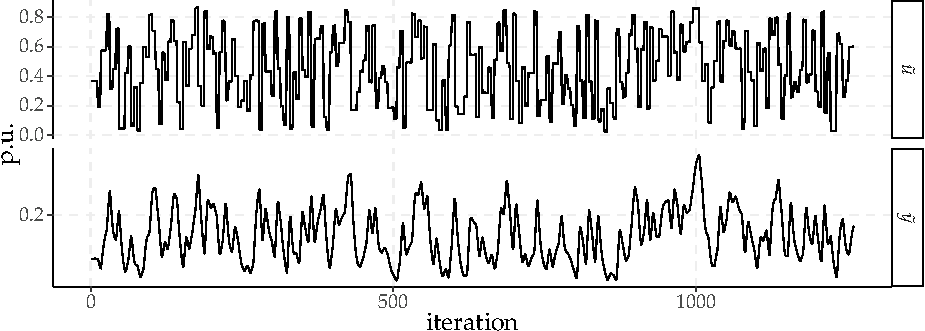
\includegraphics[width=\textwidth]{Figs/Cap5/ex53_sample_data.tex.pdf}
  \caption{Entrada e saída do aquecedor, em p.u.}
  \label{fig:ex53_samp_data}
\end{figure}
 % O período de amostragem original é de 12 segundos, porém, por simplicidade, será considerado aqui que este período de amostragem é de um segundo, $T_s =1$ s. Isto não afeta em nada os resultados a serem obtidos para fins deste exemplo numérico. Fazendo esta simplificação considera-se um modelo de referência dado por um sistema de primeira ordem, com atraso de transporte de 3 segundos e com constante de tempo de 10 segundos, resultando na seguinte função de transferência no tempo contínuo
The original sampling period is 12 seconds, however, for simplicity, it will be considered here that this sampling period is one second, $T_s =1$ s. This has no effect on the results to be obtained for the purposes of this numerical example. Making this simplification, it is considered a reference model given by a first order system, with a transport delay of 3 seconds and a time constant of 10 seconds, resulting in the following transfer function in continuous time
\begin{equation}
   M(s) = \frac{e^{-\tau_d s}}{\tau s-1},
\label{eq:}
\end{equation}
% em que $\tau = 10$ é a constante de tempo desejada e $\tau_d = 3$ é o atraso de transporte. A versão discreta deste modelo pode ser escrita como:
where $\tau = 10$ s is the desired time constant and $\tau_d = 3$ s is the transport delay. A discrete version of this model is given by
 \begin{equation}
   M(z) = \frac{1-e^{-T_s/\tau}}{(z-e^{-Ts/\tau})z^{\tau_d/Ts-1}}.
   \label{eq:ex53_MRcont}
 \end{equation}

 % Desconsiderando ruídos no processo, o procedimento RaCSS é aplicado afim de se obter um controlador que resulte em um sistema em malha fechada que se comporte de acordo com um modelo de referência dado.
 Disregarding noise in the process, the RaCSS procedure is applied in order to obtain a controller that results in a closed-loop system that behaves according to a given reference model.
 % Considera-se como regressores candidatos todos os regressores formados por monômios até 8 atrasos em $\tilde{u}$ (sinal de saída do controlador) e em $\tilde{e}$ (erro virtual).
 It is considered all regressors formed by monomials up to 8 delays in $\tilde{u}$ (controller output signal) and $\tilde{e}$ (virtual error) as candidate regressors to RaCSS.
 % Os parâmetros adotados no algorítmo RaCSS são apresentados na \ref{tab:exp53_param}, onde $\alpha$ é o fator de acoplamento dado em \eqref{eq:Jracss} e os significados dos outros símbolos são os mesmos da \ref{tab:exp51_param}.
 The parameters adopted in the RaCSS algorithm are presented in Table \ref{tab:exp53_param}, where xxxxxxxx is the factor given in \eqref{eq:Jracss} and the meanings of the other symbols are the same as presented in Table \ref{tab:exp51_param} .

\begin{table}[htpb]
  \centering
  \caption{Parameters used in the RaMSS algorithm of the example ~\ref{ex:53}}\label{tab:exp53_param}
  \begin{tabular}{c|c|c|c|c|c|c|c|c|c|c}
    $o$ & $n_{\tilde{e}}$ & $n_{\tilde{u}}$ & $ N_p$ & $ iter_{\max} $ & $K$ & $\gamma_0$ &  $\mu_{\min}$ & $\mu_{\max}$ & $\nu$ & $a$\\
    \hline
     $ 2 $ & $8$ & $8$ & $100$ & $200$ & $1$ & $2$ & $0.01$ & $1$ & $0$ & $0.5$ \\
  \end{tabular}
\end{table}

% Uma evolução típica para os RIPs, após 200 iterações é mostrada na Figura \ref{fig:ex53_rips}.
A typical evolution for the RIPs, after 200 iterations is shown in Figure \ref{fig:ex53_rips}.

  \begin{figure}[htpb]
    \centering
    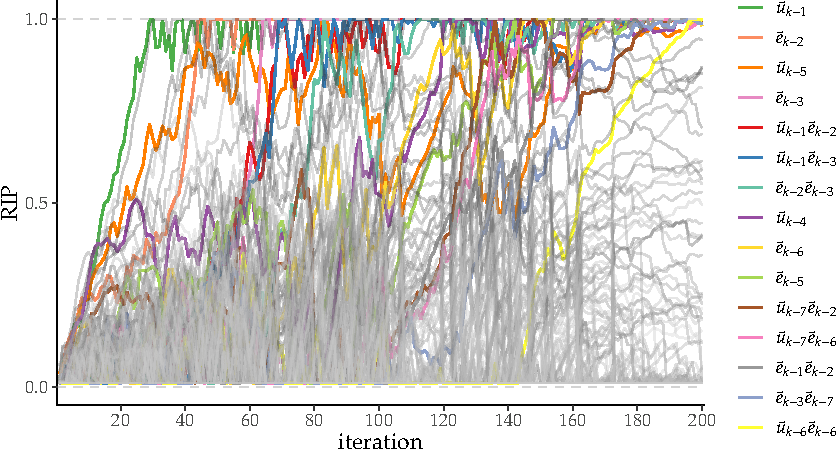
\includegraphics[width=\textwidth]{Figs/Cap5/ex53_RIPs.tex.pdf}
    \caption{RIPs evolution for example \ref{ex:53}.}
    \label{fig:ex53_rips}
  \end{figure}

  % Nota-se um comportamento bem menos regular com aqueles obtidos no Exemplo \ref{ex:52}. Ao final das 200 iterações, 15 regressores são selecionados. Apesar de ainda existirem outros regressores que ainda não convergiram para o valor mínimo e máximo, um certo grau de classificação já pode ser obtido a partir dos resultados. Ressalta-se que são um total de 171 possíveis regressores, o que resulta em um total de, aproximadamente, $2^{171}$ modelos possíveis.
  There is a much less regular behavior with those obtained in Example \ref{ex:52}. At the end of the 200 iterations, 15 regressors are selected. Although there are still other regressors that have not yet converged to the minimum and maximum value, and a certain degree of classification can already be obtained from the results. It should be noted that there are a total of 171 possible regressors, which results in a total of approximately $2^{171}$ possible models.

  % A resposta em malha fechada considerando-se os primeiros 15, 19 e 27 regressores é mostrada na Figura \ref{fig:ex31_resp_temporal}.
  The closed loop response considering the first 15, 19 and 27 regressors is shown in Figure \ref{fig:ex31_resp_temporal}.
  The MAPE, MSTE and $J_r$ index values (see \eqref{eq:MSTE} and \eqref{eq:Jracss}) are presented in Table \ref{tab: exp53_mape}.

  \begin{figure}[htpb]
  \sbox0{\blacksolidlinethin} \sbox1{\bluedashedline} \sbox2{\greendashdottedline} \sbox3{\reddashedline} \sbox4{\blackdottedline} 
    \centering
    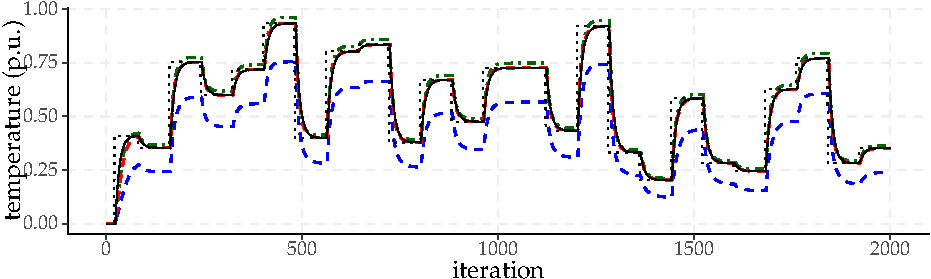
\includegraphics[width=\textwidth]{Figs/Cap5/ex53_resp_temp.tex.pdf}
    \caption{Closed loop response for controllers obtained using the first 15 (\usebox1), 19 (\usebox2) and 27 (\usebox3) RIPs obtained using RaCSS, together with the reference signal (\usebox4) and the reference model response (\usebox0).}
    \label{fig:ex31_resp_temporal}
  \end{figure}

  % Os valores do MAPE, do MSTE e do índice $J_r$ (vide \eqref{eq:MSTE} e \eqref{eq:Jracss}) são apresentados na Tabela \ref{tab:exp53_mape}.


  % Observa-se que a ao se considerar 27 regressores a resposta fica praticamente idêntica a desejada, com um valor MAPE de apenas 2.14. Nenhuma análise posterior foi feita sobre os parametros classificados. Em uma nova análise pretende-se separar os regressores selecionados e proceder novamente com o procedimento RaCSS, mas desta vez, somente com estes regressores já pré-selecionados.
  It is observed that when considering 27 regressors the answer is practically identical to the desired one, with a MAPE value of only 2.14. No further analysis was done on the classified parameters. In a new analysis, we intend to separate the selected regressors and proceed again with the RaCSS procedure, but this time, only with these pre-selected regressors.

\begin{table}[htpb]
  \centering
  \caption{Parameters used in the RaMSS algorithm of the example ~\ref{ex:53}}\label{tab:exp53_mape}
  \begin{tabular}{c|c|c|c}
     & $MAPE$ & $MSTE$ & $J_s$ \\
    \hline
    15 & 69.02 & 0.2142 & 0.8072 \\
    19 & 9.59 & 0.0050 & 0.9950 \\
    27 & 2.14 & 0.00116 & 0.9988 \\
  \end{tabular}
\end{table}


\end{exmp}


